\documentclass[conference]{IEEEtran}
\IEEEoverridecommandlockouts
\usepackage[T1]{fontenc}
\usepackage{cite}
\usepackage{amsmath,amssymb}
\usepackage{graphicx}
\usepackage{booktabs}
\usepackage{array}
\usepackage{multirow}
\usepackage{xcolor}
\usepackage{url}
\usepackage[hidelinks]{hyperref}
\def\BibTeX{{\rm B\kern-.05em{\sc i\kern-.025em b}\kern-.08em
    T\kern-.1667em\lower.7ex\hbox{E}\kern-.125emX}}
\newcommand{\pp}{\,pp}

\begin{document}

\title{Drivers of Subgroup Abstention in Selective Chest X-Ray AI: The Roles of Annotation Bias and Domain Shift}

\author{
\IEEEauthorblockN{Bara' Afanah}
\IEEEauthorblockA{\textit{Computer Engineering Department} \\
\textit{Faculty of Engineering}\\
\textit{An-Najah National University}, Nablus, Palestine \\
s12323988@stu.najah.edu}
\and
\IEEEauthorblockN{Ahmad Shanti}
\IEEEauthorblockA{\textit{Computer Science Department} \\
\textit{Faculty of IT \& Artificial Intelligence}\\
\textit{An-Najah National University}, Nablus, Palestine \\
s12326330@stu.najah.edu}
\and
\IEEEauthorblockN{Adel Ibdah}
\IEEEauthorblockA{\textit{Computer Engineering Department} \\
\textit{Faculty of Engineering}\\
\textit{An-Najah National University}, Nablus, Palestine \\
s12323227@stu.najah.edu}
\and
\IEEEauthorblockN{Basil Ibdah}
\IEEEauthorblockA{\textit{Doctor of Medicine Department} \\
\textit{Faculty of Medicine and Allied Medical Sciences}\\
\textit{An-Najah National University}, Nablus, Palestine \\
s12240294@stu.najah.edu}
}

\maketitle

\begin{abstract}
Selective classification lets a chest X-ray model abstain on uncertain cases and defer them to a radiologist. A low abstention rate in a patient subgroup is often read as a sign that the model handles that subgroup well, but it can also mean that the model is confidently wrong. We ask which upstream problem drives subgroup differences in abstention: a disease signal that is intrinsically weaker in the subgroup, underdiagnosis in the training labels, or domain shift at deployment. A controlled simulation switches each driver, and subgroup separability, on independently in a $2^4$ factorial design, and we monitor the silent-miss rate, the share of diseased patients who are missed and not deferred, which we relate formally to the false-negative rate and coverage. The drivers moved abstention in opposite directions: a weaker signal raised the subgroup's abstention by 6.7 percentage points (pp), while label bias and shift lowered it. With all four active, the abstention gap was +1.4\pp{} (95\% CI +1.0 to +1.9) but the silent-miss gap was +13.9\pp{} (+12.7 to +15.1). The pattern held under subtle-case mislabelling, nonlinear features with a neural network, and other coverage targets. On 637 real radiographs encoded by a pretrained DenseNet-121, injected label bias widened the silent-miss gap only when the group was identifiable from the embeddings (female patients +6.0\pp; random group 0.0\pp), and a scanner-like shift cut female patients' abstention from 23\% to 2\% while errors on accepted cases rose. Equalising abstention with group thresholds did not reduce silent misses, whereas per-group recalibration on a small clean-label audit set removed most of the gap caused by label bias and shift. Equal abstention rates are therefore not evidence of fairness.
\end{abstract}

\begin{IEEEkeywords}
selective classification, abstention, algorithmic fairness, chest radiography, label bias, underdiagnosis, domain shift
\end{IEEEkeywords}

%=====================================================================
\section{Introduction}

Deep learning models that read chest radiographs are increasingly proposed for triage and reporting. A common safeguard is selective classification: the model makes a prediction only when its confidence passes a threshold and defers the remaining cases to a human reader \cite{geifman2017}. Deferral is attractive because it concentrates the model's mistakes in the cases a radiologist will see anyway.

Abstention is not necessarily spread evenly across patients. Jones et al. showed that selective classification can widen accuracy gaps between groups, and that adding abstention can even lower one group's accuracy \cite{jones2021}. In chest X-ray AI, subgroup performance gaps have been traced to several upstream causes. Classifiers trained on labels mined from clinical records underdiagnose some patient groups more than others \cite{seyyedkalantari2021}, and report-labelling tools themselves perform differently across age groups \cite{santomartino2024}. Models also lose accuracy when moved between hospitals \cite{zech2018}, and public datasets combine label-quality problems with domain shift \cite{rafferty2025}. What has not been examined is how each of these causes reaches the abstention mechanism. If they push abstention in different directions, a monitor that compares abstention rates across subgroups could report parity while one subgroup is being harmed.

We study this question first with a controlled simulation, because in real datasets the causes occur together and the true labels are unknown, and then test the main mechanisms on real radiographs with a pretrained deep network. Our contributions are:
\begin{itemize}
\item a factorial simulation that separates four drivers of subgroup harm in a selective classifier: an intrinsic disease-signal gap, annotation bias, subgroup separability and domain shift;
\item the silent-miss rate as a monitoring target, with its exact relation to the false-negative rate, selective sensitivity and coverage, and evidence that it is not implied by any of them;
\item evidence that the drivers move abstention in opposite directions, that label bias acts only on separable subgroups, that some shifts raise error without raising abstention, and that audits with biased labels misstate the gap, with robustness checks and a replication of the key mechanisms on 637 real radiographs;
\item a test of two mitigations, showing that equalising abstention does not help while recalibration on a small clean-label audit set does.
\end{itemize}

%=====================================================================
\section{Related Work}

\subsection{Selective Classification and Group Fairness}
Geifman and El-Yaniv showed how to add a reject option to an already-trained deep network by choosing a confidence threshold so that the error on accepted cases stays below a target level with high probability \cite{geifman2017}. Such thresholds are set on average performance. Jones et al. found that, while abstention improves average accuracy, it can magnify existing accuracy gaps between groups and, in some groups, lower accuracy as abstention increases \cite{jones2021}. They linked this to the distribution of model confidence and proposed training models to perform equally across groups at full coverage. Their analysis treats the full-coverage gap as given and does not ask where it comes from, which is the question we address. Closer to deployment, a recent preprint proposes a fairness-aware framework that routes medical images to a model, a human expert, or both, and accounts for subgroup-dependent reliability without using sensitive attributes at test time \cite{zhang2026}. Such systems still rely on some signal of when the model is unreliable, and our results bear on when confidence fails to provide it.

\subsection{Annotation Bias and Subgroup Separability in Chest Radiography}
Labels in large public chest X-ray datasets are mostly extracted from radiology reports. Seyyed-Kalantari et al. trained classifiers on three such datasets and found that female, young, Black, Hispanic and Medicaid-insured patients were more often wrongly labelled healthy, and argued that labels drawn from clinical records can carry existing biases in care \cite{seyyedkalantari2021}. Santomartino et al. evaluated four report-labelling tools and found high pooled accuracy but error rates that varied with patient age, with most tools performing worst in patients over 80 \cite{santomartino2024}. Jones, Roschewitz and Glocker related subgroup separability, meaning how easily a model can tell subgroups apart, to the disparities and performance loss that follow training on systematically biased labels such as underdiagnosis \cite{jones2023}. We use separability as one of our four factors and test whether it also governs how label bias reaches abstention.

\subsection{Domain Shift and Hidden Failures}
Zech et al. found that pneumonia models often performed worse on radiographs from external hospital systems than on new data from the training hospitals, and that the models could identify which hospital and department an image came from \cite{zech2018}. Oakden-Rayner et al. showed that medical imaging models can look accurate overall while failing on unlabelled subsets of patients, and argued that such hidden stratification should be checked before deployment \cite{oakdenrayner2020}. Rafferty and Rajan, in a preprint, reviewed label quality, bias and domain shift in public chest radiography datasets and reported substantial loss of performance in cross-dataset testing \cite{rafferty2025}. These studies measure accuracy under shift; we ask how shift changes the confidence that abstention relies on, and therefore whether abstention signals the harm.


%=====================================================================
\section{Study Design}

\subsection{Data-Generating Process}
Each simulated case has 20 features standing in for an image embedding, a binary disease label $y$ with prevalence 0.30, and a subgroup $g$. Subgroup $B$ makes up 20\% of cases and subgroup $A$ the rest. Disease moves cases along the first feature direction and subgroup membership along the second:
\begin{equation}
x = z + \delta_g\,(y - \tfrac{1}{2})\,e_1 + s\,\mathbb{1}[g = B]\,e_2, \qquad z \sim \mathcal{N}(0, I_{20}),
\end{equation}
where $\delta_g$ is the disease-signal strength in subgroup $g$ and $s$ sets how separable the subgroups are. The two directions are orthogonal, so separability carries no information about disease by itself.

\subsection{The Four Drivers}
Table~\ref{tab:drivers} lists the drivers and their two levels. Annotation bias flips a share $u_B$ of subgroup $B$'s true positives to negative in the recorded labels used for training and auditing, which mimics underdiagnosis. Domain shift is applied only to subgroup $B$'s deployment cases: features are rescaled by $(1+0.15m)$ (contrast gain) and translated by $m$ along a random unit direction. All recorded labels also carry 3\% uniform label noise.

\begin{table}[t]
\centering
\caption{The four drivers and their levels in the factorial design.}
\label{tab:drivers}
\footnotesize
\begin{tabular}{@{}p{1.75cm}p{1.15cm}p{1.15cm}p{3.1cm}@{}}
\toprule
Driver & Low & High & Meaning \\
\midrule
Signal gap & $\delta_B{=}2.5$ & $\delta_B{=}1.8$ & Disease harder to see in $B$ ($\delta_A{=}2.5$) \\
Annotation bias & $u_B{=}0$ & $u_B{=}0.35$ & 35\% of $B$'s positives recorded as negative \\
Separability & $s{=}0$ & $s{=}2$ & Group detectable from features \\
Domain shift & $m{=}0$ & $m{=}1.5$ & $B$'s deployment features rescaled and translated \\
\bottomrule
\end{tabular}
\end{table}

\subsection{Selective Classifier}
The classifier is an $L_2$-regularised logistic regression ($C=1$) trained on 4,000 cases with the recorded labels. Its confidence is $\max(p, 1-p)$. The abstention threshold is the 20th percentile of confidence on a separate 2,000-case calibration set drawn from the training domain, so the system is designed to abstain on 20\% of cases. The threshold is then applied unchanged to 4,000 deployment cases, as a hospital would fix it before go-live.

\subsection{Metrics}
All metrics are computed per subgroup against the true labels unless stated otherwise, and gaps are reported as $B$ minus $A$ in percentage points (pp).
\begin{itemize}
\item \emph{Abstention rate}: share of cases deferred.
\item \emph{Selective risk}: error rate among accepted cases.
\item \emph{Silent-miss rate}: diseased cases that the model calls negative and does not defer, divided by all diseased cases in the subgroup.
\item \emph{Catch rate}: share of a subgroup's missed diseased cases that abstention intercepts.
\item \emph{Audit selective risk}: selective risk computed with the recorded, possibly biased labels, which is what a routine audit would measure.
\end{itemize}

\subsection{Relation of the Silent-Miss Rate to Standard Metrics}
\label{sec:metric}
The silent-miss rate is not a new probability, and we do not claim it as one. Let $Y=1$ denote disease, $\hat{Y}$ the model's prediction and $D=1$ deferral, all within one subgroup. Four familiar quantities and the silent-miss rate are
\begin{align}
\mathrm{FNR} &= P(\hat{Y}=0 \mid Y=1), \nonumber\\
\mathrm{FNR}_{\mathrm{sel}} &= P(\hat{Y}=0 \mid Y=1, D=0), \nonumber\\
c^{+} &= P(D=0 \mid Y=1), \nonumber\\
\mathrm{CR} &= P(D=1 \mid \hat{Y}=0, Y=1), \nonumber\\
\mathrm{SMR} &= P(\hat{Y}=0, D=0 \mid Y=1) \nonumber\\
 &= \mathrm{FNR}_{\mathrm{sel}}\, c^{+} = \mathrm{FNR}\,(1-\mathrm{CR}). \label{eq:smr}
\end{align}
Here FNR is the full-coverage false-negative rate, $\mathrm{FNR}_{\mathrm{sel}}$ is one minus the sensitivity on accepted cases, $c^{+}$ is the coverage of diseased patients, and CR is the catch rate. Equation~\eqref{eq:smr} shows that the silent-miss rate is the joint probability that a diseased patient is both missed and not referred, that is, the unflagged false-negative rate of the whole human-AI pathway.

Its value for monitoring comes from what parity in the usual metrics does \emph{not} imply. Equal overall coverage does not give equal $c^{+}$, because the two groups can differ in prevalence and in how confident the model is on their diseased cases. Equal selective sensitivity does not give equal SMR when $c^{+}$ differs, and equal full-coverage FNR does not give equal SMR when the catch rate differs. The silent-miss rate is the one quantity that equals a diseased patient's risk of leaving the system undiagnosed, and it can be estimated from the same confusion counts as the others. Section~\ref{sec:decomp} shows empirically that the gaps in these quantities can differ in size and even in sign.


\subsection{Experiments and Statistics}
The main experiment is a full $2\times2\times2\times2$ factorial design with 200 independent replicates in each of the 16 cells. Main and two-way interaction effects are estimated by ordinary least squares on $\pm1$-coded factors, with 95\% intervals from 400 bootstrap resamples within cells. We also attribute the change from the all-off to the all-on cell to the four drivers using Shapley values averaged over all 24 orderings. Three further experiments vary one driver at a time with 100 replicates per point: the underdiagnosis rate from 0 to 0.5 at two separability levels, the shift magnitude from 0 to 3 for three shift types, and the share of subgroup $B$ from 5\% to 50\%. As a robustness check, four archetype scenarios were repeated with a one-hidden-layer neural network (32 units, 30 replicates, smaller samples). Scenario means carry $t$-based 95\% confidence intervals over replicates. Software versions, seeds and settings are listed in Table~\ref{tab:repro}.

%=====================================================================
\subsection{Real Chest Radiographs}
\label{sec:realmethod}
To check the mechanisms on real images and a modern deep model, we used the public COVID-19 image data collection \cite{cohen2020covid}, which gathers radiographs from many hospitals and publications. We kept frontal X-rays with recorded sex and a confirmed finding: 637 images from 381 patients, 241 of them female, with 432 COVID-19 images and 205 images with other findings (other pneumonias, tuberculosis or no finding). The task was COVID-19 versus other findings, and female patients formed subgroup $B$. Each image was encoded once by a DenseNet-121 pretrained on seven public chest X-ray datasets and distributed with TorchXRayVision \cite{cohen2021xrv}; we used its frozen 1024-dimensional embedding and trained an $L_2$-regularised logistic regression on top, with the same 20\% abstention rule as in the simulation. We drew 300 random patient-level splits (60\% training, 20\% calibration, 20\% deployment), so no patient appeared in more than one part.

Separability was measured directly: a logistic regression predicted sex from the embeddings with a patient-grouped five-fold AUC of 0.71. Label bias was injected by relabelling 35\% of female COVID-19 training images as negative, and evaluated against the original labels. As a control with no separability, the same bias was injected into a \emph{random} group of patients of the same size, which the images cannot reveal. Two real acquisition shifts were tested on female deployment images only. In the \emph{view shift}, female anteroposterior supine (portable, mostly intensive-care) radiographs were withheld from training and calibration and used only at deployment. In the \emph{scanner shift}, female deployment images were altered with a tone curve ($\gamma = 1.8$), lower contrast, blur and noise, then re-encoded by the network. Because each deployment set held only about 48 female patients, we report means over the 300 splits together with the range covering 95\% of splits and the share of splits in which a change had the stated sign.


\section{Results}

\subsection{The Drivers Push Abstention in Opposite Directions}

With no driver active the system behaved as designed: both subgroups had 19.9\% abstention and 3.8--3.9\% selective risk (Table~\ref{tab:scen}). Each driver then moved subgroup $B$'s abstention rate, but not in the same direction (Fig.~\ref{fig:shapley}). A weaker disease signal raised it by 6.7\pp. Domain shift lowered it by 3.5\pp, and annotation bias and separability each lowered it by about 0.9\pp. The silent-miss gap, in contrast, rose under every driver.

\begin{figure*}[t]
\centering
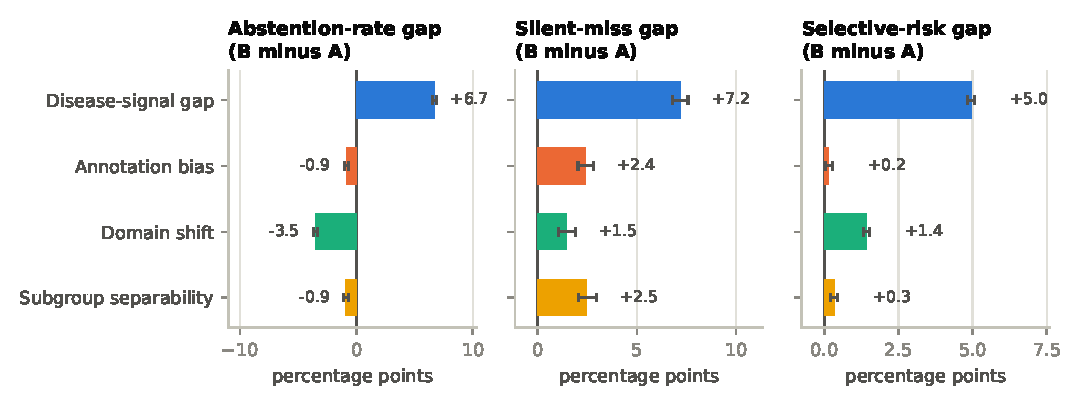
\includegraphics[width=0.92\textwidth]{figs/fig1_shapley.pdf}
\caption{Shapley attribution of the change from the all-off to the all-on factorial cell to each driver, for three subgroup gaps ($B$ minus $A$, pp). Bars are means over 200 replicates per cell; whiskers are 95\% bootstrap intervals.}
\label{fig:shapley}
\end{figure*}

\begin{table*}[t]
\centering
\caption{Subgroup outcomes in selected factorial cells (logistic regression, 200 replicates each). Gaps are $B$ minus $A$ with 95\% confidence intervals.}
\label{tab:scen}
\footnotesize
\setlength{\tabcolsep}{4pt}
\begin{tabular}{@{}lccccccc@{}}
\toprule
Scenario & \shortstack{Abstain\\$A$ (\%)} & \shortstack{Abstain\\$B$ (\%)} & \shortstack{Abstention\\gap (pp)} & \shortstack{Sel.\ risk\\$A$ / $B$ (\%)} & \shortstack{Silent misses\\in $B$ (\%)} & \shortstack{Silent-miss\\gap (pp)} & \shortstack{Misses caught\\in $B$ (\%)} \\
\midrule
All drivers off & 19.9 & 19.9 & $0.0$ [$-0.2$, $+0.2$] & 3.8 / 3.9 & 7.0 & $+0.3$ [$+0.1$, $+0.6$] & 63 \\
Signal gap only & 18.5 & 26.3 & $+7.8$ [$+7.5$, $+8.0$] & 4.0 / 8.8 & 14.0 & $+6.4$ [$+6.1$, $+6.8$] & 54 \\
Annotation bias + separability & 20.2 & 18.9 & $-1.3$ [$-1.5$, $-1.1$] & 3.9 / 5.0 & 12.3 & $+4.1$ [$+3.8$, $+4.5$] & 59 \\
Domain shift only & 20.0 & 16.5 & $-3.5$ [$-3.8$, $-3.2$] & 3.7 / 5.0 & 8.6 & $+2.0$ [$+1.4$, $+2.7$] & 54 \\
Annotation + separability + shift & 20.3 & 15.7 & $-4.6$ [$-4.9$, $-4.3$] & 3.9 / 5.9 & 13.9 & $+5.8$ [$+5.0$, $+6.6$] & 50 \\
All four drivers & 19.2 & 20.6 & $+1.4$ [$+1.0$, $+1.9$] & 4.1 / 11.1 & 22.4 & $+13.9$ [$+12.7$, $+15.1$] & 42 \\
\bottomrule
\end{tabular}
\end{table*}

The opposing effects cancel. With all four drivers on, $B$ abstained only 1.4\pp{} more than $A$, close enough to pass as fair on a monitoring dashboard. Yet 22.4\% of $B$'s diseased cases were missed and accepted without deferral, against 8.5\% in $A$, and abstention caught 42\% of $B$'s missed cases compared with 63\% at baseline.

The fifth row of Table~\ref{tab:scen} is the most worrying case. Without any intrinsic signal gap, $B$ abstained 4.6\pp{} \emph{less} than $A$, which a reviewer might read as the model being more certain about $B$, while $B$'s silent-miss rate was 5.8\pp{} higher.

The signal gap is the only driver that behaves as the selective-classification literature predicts \cite{jones2021}. At full coverage $B$'s error was 1.72 times $A$'s (16.3\% vs.\ 9.5\%); at 80\% target coverage it was 2.19 times (8.8\% vs.\ 4.0\%). Abstention lowered both error rates but widened the ratio.

\subsection{Annotation Bias Harms Only a Separable Subgroup}

When group membership could not be read from the features, underdiagnosis in $B$'s labels left $B$ almost untouched: even at an underdiagnosis rate of 0.5, the silent-miss gap stayed within 0.2\pp{} of zero (Fig.~\ref{fig:dose}, top). Without a group signal, the model cannot apply the bias to $B$ alone, so its effect is spread over the whole population. Once the subgroup was separable, the same label bias produced a dose-response: the silent-miss gap rose steadily to 6.6\pp{} while $B$'s abstention rate fell by 2.1\pp. In the factorial model this appears as an annotation $\times$ separability interaction of +2.4\pp{} [+2.1, +2.7] on the silent-miss gap, about as large as either main effect.

\begin{figure*}[t]
\centering
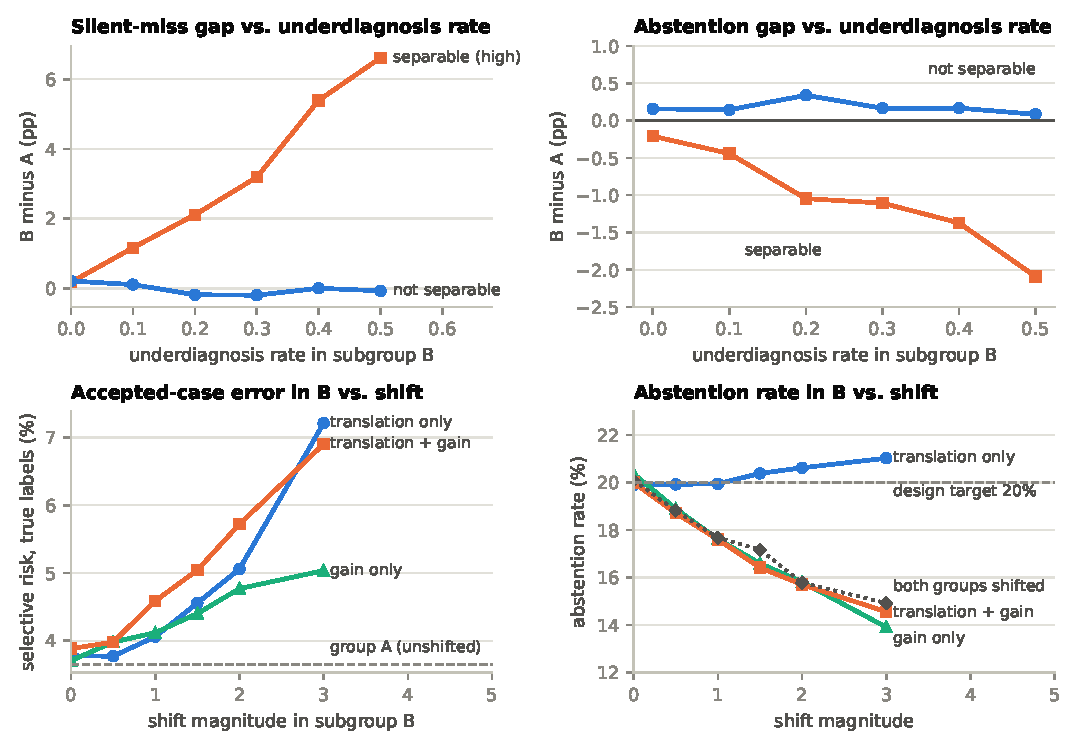
\includegraphics[width=0.86\textwidth]{figs/fig2_dose.pdf}
\caption{Dose-response experiments (100 replicates per point). Top: silent-miss gap and abstention gap as the underdiagnosis rate in $B$ increases, with and without subgroup separability. Bottom: selective risk (true labels) and abstention rate in $B$ as domain shift grows, for three shift types; dashed lines mark group $A$ and the 20\% design target.}
\label{fig:dose}
\end{figure*}

The size of the subgroup mattered for label bias but not for shift (Table~\ref{tab:minority}). The annotation-bias silent-miss gap grew from 1.1\pp{} when $B$ was 5\% of the population to 7.0\pp{} at 50\%, whereas the shift-induced gap stayed between 1.6 and 1.9\pp. A plausible explanation is that a larger subgroup contributes more biased labels to training, so the model learns a subgroup-specific boundary more firmly.

\begin{table}[t]
\centering
\caption{Silent-miss gap ($B$ minus $A$, pp) by share of subgroup $B$ (100 replicates per point).}
\label{tab:minority}
\footnotesize
\begin{tabular}{@{}ccc@{}}
\toprule
Share of $B$ & Annotation bias + separability & Domain shift \\
\midrule
5\% & +1.1 & +1.7 \\
10\% & +2.3 & +1.6 \\
20\% & +4.3 & +1.7 \\
30\% & +5.5 & +1.9 \\
50\% & +7.0 & +1.6 \\
\bottomrule
\end{tabular}
\end{table}

\subsection{Domain Shift Harms Without Raising Abstention}

Shift that affected only subgroup $B$ never raised $B$'s abstention by more than about one point, but it always raised the error on cases the system accepted (Fig.~\ref{fig:dose}, bottom). The type of shift decided what happened to abstention (Table~\ref{tab:shift}). Contrast gain stretches cases away from the decision boundary, so the model becomes more confident and abstains less, by 6\pp{} at the largest shift. Translation moves cases without making them look uncertain, so abstention stayed near its 20\% target while selective risk almost doubled. In neither case does the abstention rate give a warning.

\begin{table}[t]
\centering
\caption{Abstention and selective risk in $B$ at the largest shift ($m=3$; true labels, 100 replicates per point).}
\label{tab:shift}
\footnotesize
\begin{tabular}{@{}lcc@{}}
\toprule
Shift type in $B$ & Abstention in $B$ (\%) & Selective risk in $B$ (\%) \\
\midrule
None ($m=0$) & 19.9--20.4 & 3.7--3.9 \\
Translation only & 21.0 & 7.2 \\
Contrast gain only & 13.9 & 5.0 \\
Translation + gain & 14.6 & 6.9 \\
\bottomrule
\end{tabular}
\end{table}

When the same shift hit both groups, abstention fell to 14.9\% and selective risk rose to 6.6--6.7\% in each, with no gap between them. Shift is therefore a fairness problem specifically when it is group-specific, for example when one subgroup is mostly imaged on different equipment or at a different site.

\subsection{Biased-Label Audits, Risk-Coverage Curves, and a Second Model}

A hospital can audit a deployed model only against the labels it has. When those labels carry the same underdiagnosis the model was trained on, the audit misstates the subgroup gap (Table~\ref{tab:arch}). In the annotation-bias scenario the audit put $B$'s selective-risk gap at +5.1\pp{} when the true gap was +1.2\pp. The audit inflates the error because it scores the model's correct detections in $B$ as false positives. It also cannot see the misses that matter most: by construction, 35\% of $B$'s diseased cases are recorded as negative, so a model that misses them agrees with the record. Shift without label bias was audited accurately (+1.3\pp{} audited vs.\ +1.4\pp{} true).

\begin{table*}[t]
\centering
\caption{Subgroup gaps ($B$ minus $A$, pp, 95\% CI) in four archetype scenarios for logistic regression (LR, 100 replicates) and a one-hidden-layer network (MLP, 30 replicates). Annotation bias uses $u_B = 0.35$ with $s = 2$; shift uses $m = 1.5$.}
\label{tab:arch}
\footnotesize
\begin{tabular}{@{}llcccc@{}}
\toprule
Scenario & Model & Abstention gap & Silent-miss gap & \shortstack{Selective-risk gap\\(true labels)} & \shortstack{Selective-risk gap\\(biased-label audit)} \\
\midrule
\multirow{2}{*}{Baseline} & LR & $+0.3$ [$-0.1$, $+0.6$] & $-0.1$ [$-0.5$, $+0.2$] & $0.0$ [$-0.2$, $+0.2$] & $0.0$ [$-0.3$, $+0.2$] \\
 & MLP & $+0.2$ [$-0.6$, $+1.0$] & $0.0$ [$-1.1$, $+1.0$] & $-0.1$ [$-0.6$, $+0.3$] & $-0.2$ [$-0.8$, $+0.3$] \\
\midrule
\multirow{2}{*}{Annotation bias} & LR & $-1.4$ [$-1.8$, $-1.1$] & $+4.8$ [$+4.3$, $+5.4$] & $+1.2$ [$+1.1$, $+1.4$] & $+5.1$ [$+4.8$, $+5.4$] \\
 & MLP & $+0.9$ [$+0.1$, $+1.6$] & $+6.8$ [$+5.3$, $+8.3$] & $+1.6$ [$+1.0$, $+2.2$] & $+4.5$ [$+3.8$, $+5.2$] \\
\midrule
\multirow{2}{*}{Domain shift} & LR & $-3.3$ [$-3.7$, $-2.8$] & $+1.8$ [$+0.9$, $+2.7$] & $+1.4$ [$+1.1$, $+1.6$] & $+1.3$ [$+1.0$, $+1.6$] \\
 & MLP & $-3.4$ [$-4.5$, $-2.2$] & $+3.0$ [$+0.7$, $+5.3$] & $+1.8$ [$+1.3$, $+2.2$] & $+1.9$ [$+1.3$, $+2.5$] \\
\midrule
\multirow{2}{*}{Both} & LR & $-4.6$ [$-4.9$, $-4.2$] & $+6.6$ [$+5.2$, $+8.0$] & $+2.3$ [$+1.9$, $+2.7$] & $+6.9$ [$+6.5$, $+7.2$] \\
 & MLP & $-2.5$ [$-3.5$, $-1.4$] & $+9.3$ [$+6.0$, $+12.6$] & $+3.0$ [$+2.1$, $+3.8$] & $+6.4$ [$+5.5$, $+7.3$] \\
\bottomrule
\end{tabular}
\end{table*}

Risk-coverage curves show that these gaps are not an artefact of the 80\% operating point (Fig.~\ref{fig:rc}). Under annotation bias, shift, or both, $B$'s curve lies above $A$'s at every coverage level from 50\% to 100\%. Abstaining more narrows the absolute gap but does not close it.

\begin{figure*}[t]
\centering
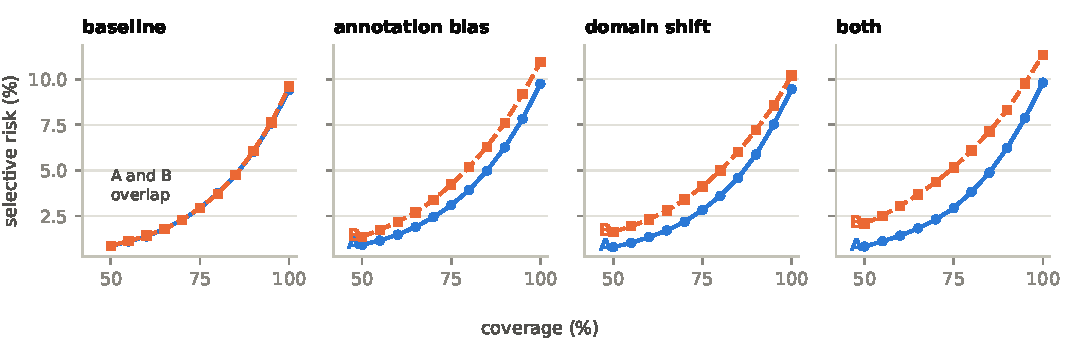
\includegraphics[width=0.92\textwidth]{figs/fig3_riskcov.pdf}
\caption{Risk-coverage curves per subgroup (true labels, logistic regression, 100 replicates) for the four archetype scenarios. At baseline the two curves coincide.}
\label{fig:rc}
\end{figure*}

The neural network reproduced the main pattern: silent misses in $B$ were higher under every driver, and larger than with logistic regression. One result depended on the model. Under annotation bias alone, the network abstained slightly more on $B$ (+0.9\pp) while logistic regression abstained less ($-1.4$\pp), so the sign of the abstention change caused by label bias should not be taken as general. The effect of shift on abstention was the same for both models.

%=====================================================================
\subsection{What the Silent-Miss Rate Adds Over Standard Metrics}
\label{sec:decomp}
To test whether the silent-miss rate carries information beyond familiar metrics, a second simulation run (60 replicates per scenario, same design) recorded all quantities of Eq.~\eqref{eq:smr} per subgroup (Table~\ref{tab:decomp}). The gaps disagree in ways that matter for monitoring. With a signal gap, the full-coverage FNR gap (+10.9\pp) overstated the harm of the deployed pathway, because deferral sent many of $B$'s errors to a radiologist; the silent-miss gap was +6.3\pp. Under domain shift the opposite happened: the FNR gap was null ($-0.3$\pp) and the selective-FNR gap was not significant, yet $B$'s diseased patients were accepted more often ($c^{+}$ +6.8\pp), so the silent-miss gap was positive (+1.2\pp{} [+0.2, +2.3]). At 70\% target coverage the FNR gap under shift even favoured $B$ ($-2.9$\pp{} [$-5.1$, $-0.8$]) while the silent-miss gap did not (+0.7\pp{} [$-0.3$, +1.6]). With all four drivers, abstention was at parity (+0.1\pp), and the selective-FNR gap (+26.7\pp) exceeded the silent-miss gap (+16.6\pp) because it conditions on acceptance. No single standard metric tracked the patient-level risk of an unflagged miss across scenarios.

\begin{table*}[t]
\centering
\caption{Subgroup gaps ($B$ minus $A$, pp, 95\% CI) in abstention and in the quantities of Eq.~\eqref{eq:smr}; logistic regression, 80\% target coverage, 60 replicates per scenario.}
\label{tab:decomp}
\footnotesize
\begin{tabular}{@{}lccccc@{}}
\toprule
Scenario & Abstention & FNR (full coverage) & Selective FNR & Coverage of diseased, $c^{+}$ & Silent-miss rate \\
\midrule
Baseline & $-0.1$ {\scriptsize[-0.5, +0.3]} & $0.0$ {\scriptsize[-0.6, +0.7]} & $0.0$ {\scriptsize[-0.7, +0.7]} & $+0.5$ {\scriptsize[-0.3, +1.3]} & $0.0$ {\scriptsize[-0.4, +0.5]} \\
Signal gap & $+7.1$ {\scriptsize[+6.6, +7.6]} & $+10.9$ {\scriptsize[+10.3, +11.6]} & $+11.3$ {\scriptsize[+10.5, +12.1]} & $-6.9$ {\scriptsize[-7.8, -6.0]} & $+6.3$ {\scriptsize[+5.7, +6.9]} \\
Annotation bias & $-1.6$ {\scriptsize[-2.0, -1.2]} & $+8.1$ {\scriptsize[+7.2, +9.1]} & $+9.0$ {\scriptsize[+7.9, +10.1]} & $-5.3$ {\scriptsize[-6.3, -4.3]} & $+4.6$ {\scriptsize[+4.0, +5.3]} \\
Domain shift & $-3.3$ {\scriptsize[-3.8, -2.7]} & $-0.3$ {\scriptsize[-2.2, +1.5]} & $+1.2$ {\scriptsize[-0.4, +2.8]} & $+6.8$ {\scriptsize[+5.1, +8.5]} & $+1.2$ {\scriptsize[+0.2, +2.3]} \\
Annotation + shift & $-4.6$ {\scriptsize[-5.1, -4.1]} & $+6.2$ {\scriptsize[+3.6, +8.8]} & $+9.5$ {\scriptsize[+6.4, +12.6]} & $+3.8$ {\scriptsize[+2.3, +5.4]} & $+6.4$ {\scriptsize[+4.6, +8.2]} \\
All four & $+0.1$ {\scriptsize[-0.7, +0.9]} & $+20.8$ {\scriptsize[+18.1, +23.4]} & $+26.7$ {\scriptsize[+23.2, +30.2]} & $-1.7$ {\scriptsize[-2.8, -0.7]} & $+16.6$ {\scriptsize[+14.4, +18.8]} \\
\bottomrule
\end{tabular}
\end{table*}

\subsection{Robustness to the Simulation's Assumptions}
We repeated the archetype scenarios under four changes to the assumptions (Table~\ref{tab:robust}): underdiagnosis concentrated on the subtle cases (the 35\% of $B$'s positives with the weakest disease evidence are mislabelled, rather than a random 35\%); features passed through a random nonlinear map and classified by a two-layer neural network; and target coverage of 90\% or 70\% instead of 80\%. The silent-miss gap under annotation bias stayed between +2.7 and +6.5\pp, and with all four drivers between +10.7 and +17.2\pp, while the abstention gap in that scenario stayed within 2.7\pp{} of parity. Domain shift lowered $B$'s abstention in every variant ($-1.6$ to $-4.4$\pp); its silent-miss gap was positive in all five variants but its confidence interval excluded zero only in three (main, subtle cases, nonlinear). As in the factorial run, the direction of the abstention change under annotation bias depended on the model: it was negative for logistic regression and positive for the neural network.

\begin{table}[t]
\centering
\caption{Robustness: abstention gap and silent-miss gap ($B$ minus $A$, pp) under changed assumptions (60 replicates; 30 for the MLP).}
\label{tab:robust}
\footnotesize
\setlength{\tabcolsep}{3pt}
\begin{tabular}{@{}lcccccc@{}}
\toprule
 & \multicolumn{2}{c}{Annotation bias} & \multicolumn{2}{c}{Domain shift} & \multicolumn{2}{c}{All four} \\
Variant & Abst. & SMR & Abst. & SMR & Abst. & SMR \\
\midrule
Main setting & $-1.6$ & $+4.6$ & $-3.3$ & $+1.2$ & $+0.1$ & $+16.6$ \\
Subtle cases mislabelled & $-1.3$ & $+3.9$ & $-3.2$ & $+1.7$ & $+1.3$ & $+13.4$ \\
Nonlinear + MLP & $+2.4$ & $+6.5$ & $-2.1$ & $+4.2$ & $+2.7$ & $+15.4$ \\
Coverage 90\% & $-0.5$ & $+5.8$ & $-1.6$ & $+0.5$ & $+0.7$ & $+17.2$ \\
Coverage 70\% & $-2.5$ & $+2.7$ & $-4.4$ & $+0.7$ & $+1.5$ & $+10.7$ \\
\bottomrule
\end{tabular}
\end{table}

\subsection{Testing Two Mitigations}
We compared the global threshold with two remedies (Table~\ref{tab:mitig}). The first gives each subgroup its own threshold so that both abstain on 20\% of their calibration cases, which is what a team would do to equalise abstention rates. The second recalibrates the model's probabilities separately per subgroup (Platt scaling) on a small audit set of 600 deployment cases with correct labels, then applies one threshold set for 20\% abstention on that audit set.

\begin{table*}[t]
\centering
\caption{Abstention gap and silent-miss gap ($B$ minus $A$, pp) under three deferral policies, and abstention rates of $B$ / $A$ (\%) after audit recalibration (logistic regression, 60 replicates per scenario).}
\label{tab:mitig}
\footnotesize
\begin{tabular}{@{}lccccccc@{}}
\toprule
 & \multicolumn{2}{c}{Global threshold} & \multicolumn{2}{c}{Group-specific thresholds} & \multicolumn{2}{c}{Audit recalibration} & Abstention \\
Scenario & Abst. gap & SMR gap & Abst. gap & SMR gap & Abst. gap & SMR gap & $B$ / $A$ (\%) \\
\midrule
Signal gap & $+7.1$ & $+6.3$ & $-0.2$ & $+10.0$ & $+15.1$ & $+4.6$ & 32 / 17 \\
Annotation bias & $-1.6$ & $+4.6$ & $-0.3$ & $+3.9$ & $+0.6$ & $+0.2$ & 21 / 20 \\
Domain shift & $-3.3$ & $+1.2$ & $-3.9$ & $+1.5$ & $-0.5$ & $0.0$ & 20 / 20 \\
Annotation + shift & $-4.6$ & $+6.4$ & $-3.3$ & $+5.7$ & $-1.9$ & $+0.9$ & 19 / 21 \\
All four & $+0.1$ & $+16.6$ & $-3.5$ & $+19.1$ & $+14.2$ & $+4.4$ & 31 / 17 \\
\bottomrule
\end{tabular}
\end{table*}

Equalising abstention did not reduce silent misses and sometimes increased them: with a signal gap the silent-miss gap rose from +6.3 to +10.0\pp, and with all four drivers from +16.6 to +19.1\pp, because the group-specific threshold removed the extra deferrals that had been protecting $B$. Recalibration on clean audit labels removed almost all of the gap caused by annotation bias (+4.6 to +0.2\pp), domain shift (+1.2 to 0.0\pp) and the two together (+6.4 to +0.9\pp), with abstention rates staying near 20\% in both groups. When $B$'s disease signal was intrinsically weaker, recalibration narrowed the gap (+6.3 to +4.6\pp; +16.6 to +4.4\pp{} with all drivers) only by deferring many more of $B$'s cases (32\% vs.\ 17\%). In that case the remedy moves the burden to radiologists rather than removing it, which is the honest outcome when the images themselves carry less information.


\subsection{Results on Real Radiographs}
\label{sec:realres}
Table~\ref{tab:real} summarises the real-image experiment. Without any intervention, the model already served female patients worse: discrimination was lower (AUC 0.74 vs.\ 0.84), female patients were deferred more often (+4.8\pp), and their silent-miss rate was higher (+6.9\pp; positive in 84\% of splits). This is the signal-gap pattern of Section~\ref{sec:decomp}, in which abstention does point at the disadvantaged group.

\begin{table*}[t]
\centering
\caption{Real chest radiographs (637 images, 381 patients; DenseNet-121 embeddings; 300 patient-level splits). Rates and gaps are $B$ minus $A$ in pp: means over splits, with the range covering 95\% of splits. AUC is for COVID-19 detection in $B$ / $A$.}
\label{tab:real}
\footnotesize
\begin{tabular}{@{}llcccccc@{}}
\toprule
Grouping & Scenario & Abstain $B$ / $A$ (\%) & Abstention gap & Silent-miss gap & Selective-risk gap & AUC $B$ / $A$ \\
\midrule
\multirow{5}{*}{\shortstack[l]{Sex\\(AUC 0.71)}} & No intervention & 23.3 / 18.5 & $+4.8$ [$-10.7$, $+21.7$] & $+6.9$ [$-4.4$, $+20.3$] & $+11.3$ [$-7.7$, $+31.1$] & 0.74 / 0.84 \\
 & Label bias & 22.7 / 19.0 & $+3.7$ [$-11.5$, $+21.9$] & $+12.9$ [$-3.3$, $+33.3$] & $+13.1$ [$-4.8$, $+33.8$] & 0.71 / 0.82 \\
 & View shift & 10.1 / 17.6 & $-7.6$ [$-20.2$, $+2.6$] & $-0.7$ [$-7.3$, $+5.6$] & $+8.7$ [$-1.6$, $+17.5$] & 0.59 / 0.83 \\
 & Scanner shift & \phantom{0}1.7 / 18.5 & $-16.9$ [$-31.1$, $-2.6$] & $+5.7$ [$-12.3$, $+92.0$] & $+27.6$ [$+2.9$, $+53.5$] & 0.45 / 0.84 \\
 & Label bias + scanner & \phantom{0}0.6 / 19.0 & $-18.4$ [$-30.7$, $-7.5$] & $+21.0$ [$-16.4$, $+96.0$] & $+27.8$ [$+3.6$, $+55.0$] & 0.48 / 0.82 \\
\midrule
\multirow{2}{*}{\shortstack[l]{Random\\(AUC 0.5)}} & No intervention & 19.8 / 20.5 & $-0.7$ [$-17.6$, $+15.9$] & $0.0$ [$-14.4$, $+11.8$] & $+0.5$ [$-21.7$, $+21.2$] & 0.80 / 0.80 \\
 & Label bias & 19.5 / 21.2 & $-1.7$ [$-16.4$, $+12.6$] & $0.0$ [$-17.0$, $+19.1$] & $+0.4$ [$-20.3$, $+23.8$] & 0.77 / 0.77 \\
\bottomrule
\end{tabular}
\end{table*}

The two label-bias rows reproduce the separability result on real images. Injected into female patients, whom the embeddings can partly identify, label bias raised the silent-miss gap by 6.0\pp{} relative to no intervention (an increase in 81\% of splits) and raised female patients' own silent-miss rate by 10.0\pp, while their abstention rate barely moved ($-0.6$\pp). Injected into a random group of the same size, the same bias raised that group's silent-miss rate by 6.8\pp{} but raised everyone else's by the same amount, so the gap stayed at zero: the harm was spread across all patients instead of being concentrated on one group.

Both real shifts lowered female patients' abstention, as in the simulation. The scanner shift cut it from 23.3\% to 1.7\% (lower in 99\% of splits) while discrimination collapsed below chance (AUC 0.45) and the error on accepted cases rose by 16.4\pp. In this case the harm appeared mainly as confident false positives, so the silent-miss gap did not grow, but the system stopped asking for help at the moment its predictions became least reliable. The view shift lowered abstention by 13.2\pp{} (lower in 97\% of splits) and discrimination by 0.14, without a measurable rise in silent misses or selective risk; supine images in this collection have a higher COVID-19 prevalence, which makes this comparison harder to interpret. Combined with label bias, the scanner shift produced the pattern of the simulation's worst case: abstention 18.4\pp{} lower for female patients and a silent-miss gap of +21.0\pp.


%=====================================================================
\section{Discussion}

The main finding is that a subgroup's abstention rate does not show whether that subgroup is being served well. Of the four drivers, only an intrinsic signal gap made the selective model abstain more on the disadvantaged group, which is the behaviour a fairness monitor would look for. Label bias and domain shift, both documented in chest X-ray data \cite{seyyedkalantari2021,zech2018}, lowered abstention or left it unchanged. Together they can produce equal abstention rates alongside a large gap in missed disease. The real-image experiment reproduced two of these mechanisms with a pretrained deep network: label bias widened the gap only for a group the embeddings could identify, and an acquisition change made the system defer far less often for the affected group while its accuracy fell.

This changes what a deployment report should contain. We suggest three steps. First, report the silent-miss rate per subgroup alongside abstention and selective risk, since abstention parity alone is not evidence of fairness. Second, estimate silent misses on a small audit set with independently adjudicated labels; our audit experiment shows that routine labels sharing the training labels' bias can misstate the gap two- to four-fold. Third, treat a lower abstention rate in one subgroup as a prompt to check for group-specific acquisition differences or label bias, not as a sign that the model is justifiably more certain about that group.

The separability result fits the finding of Jones et al. that subgroup separability is related to how much performance a subgroup loses when a model is trained on systematically biased labels such as underdiagnosis \cite{jones2023}. Our simulation adds that the same condition also decides whether label bias reaches the abstention mechanism. Predicting a protected attribute from model embeddings is cheap, so separability could be used as a screening step when deciding how much audit effort a subgroup needs.


The mitigation experiment points the same way. Equalising abstention with subgroup-specific thresholds is the obvious fix for an abstention-parity monitor, and it did not reduce silent misses; it sometimes increased them by removing deferrals that had been protecting the subgroup. What worked was correcting the confidence score itself with a small set of clean, locally labelled cases: recalibrating per subgroup on 600 audit cases removed nearly all of the silent-miss gap caused by label bias and shift. The audit set therefore serves two purposes, measuring the harm and repairing it, which strengthens the case for collecting one at each deployment site.

\section{Limitations}

Our evidence comes in two tiers, each with limits. The simulation establishes mechanisms under stated assumptions: Gaussian features, two subgroups, one confidence score (the maximum predicted probability) and a parametric shift. The robustness checks relax some of these assumptions but not all, and the simulated effect sizes should not be read as estimates for any deployed system. The real-image experiment uses a modern pretrained network, but on a small collection assembled from many hospitals and publications, with a task (COVID-19 versus other findings) whose labels we treated as correct, label bias that we injected rather than observed, and frozen embeddings with a linear classifier instead of end-to-end fine-tuning. With about 48 female patients per deployment split, single splits vary widely, so only the averages over 300 splits should be interpreted. The scanner shift was produced by image processing rather than by a different device, and the view-shift comparison is confounded by a higher COVID-19 prevalence among supine images. We tested two mitigations, both of which assume that a correctly labelled audit set from the deployment site is available. Confirming effect sizes requires a large multi-site dataset with radiologist-adjudicated labels, which is our next step.

\section{Conclusion}

In a controlled simulation of selective chest X-ray classification, the drivers of subgroup harm moved abstention in opposite directions. A weaker disease signal raised a subgroup's abstention rate, while underdiagnosis-style label bias and group-specific domain shift lowered it or left it near target, even as missed disease accepted without deferral increased. Label bias mattered only when the subgroup was detectable from the features, a result we reproduced on real radiographs with a pretrained deep network, and audits that reused the biased labels misstated the gap. Equalising abstention did not reduce the harm, but recalibrating on a small clean-label audit set did. Abstention parity is therefore not a sufficient fairness check for selective medical AI; per-subgroup silent-miss rates on independently labelled audit data are a more direct one.

\section*{Data and Code Availability}
The simulated data are generated by our scripts; the real radiographs are from the public COVID-19 image data collection \cite{cohen2020covid} (\url{https://github.com/ieee8023/covid-chestxray-dataset}), and the pretrained network is from TorchXRayVision \cite{cohen2021xrv}. The scripts that generate every number, table and figure are provided with this paper, and rerunning them with the stated seeds reproduces the results exactly. Software versions, seeds and settings are given in Table~\ref{tab:repro}.
\begin{table}[!t]
\centering
\caption{Reproducibility details.}\label{tab:repro}
\footnotesize
\begin{tabular}{@{}p{1.7cm}p{6.1cm}@{}}
\toprule
Item & Value \\
\midrule
Software & Python 3.13.16, NumPy 2.5.3, scikit-learn 1.9.1, pandas 3.0.5, SciPy 1.18.1, Matplotlib 3.11.2 \\
Seeds & NumPy \texttt{SeedSequence} with entropy [20261018, CRC32 of cell name]; one child sequence per replicate \\
Sample sizes & 4,000 training / 2,000 calibration / 4,000 deployment per replicate (MLP: 2,000 / 1,000 / 3,000) \\
Fixed settings & 20 features, prevalence 0.30, share of $B$ 0.20, $\delta_A = 2.5$, 3\% label noise, target coverage 0.80 \\
Classifiers & Logistic regression ($C=1$); MLP, one hidden layer of 32 units \\
Replicates & Factorial 200 per cell; dose-response 100 per point; archetypes 100 (LR) and 30 (MLP) \\
Compute & About 2.5 min on 2 CPU cores for all experiments \\
\bottomrule
\end{tabular}
\end{table}


\bibliographystyle{IEEEtran}
\bibliography{refs}

\end{document}
